%%% LaTeX Template: Article/Thesis/etc. with colored headings and special fonts
%%%
%%% Source: http://www.howtotex.com/
%%% Feel free to distribute this template, but please keep to referal to http://www.howtotex.com/ here.
%%% February 2011
%%%
%%% Modified October 2015 by CDM

%%%  Preamble
% In your .tex file
% !TEX program = pdflatex 
\documentclass[11pt,letterpaper]{article}
\usepackage[margin=1.0in]{geometry}
\usepackage[T1]{fontenc}
\usepackage[bitstream-charter]{mathdesign}
\usepackage[latin1]{inputenc}					
\usepackage{amsmath}						
\usepackage{xcolor}
\usepackage{cite}
\usepackage{hyphenat}
\usepackage{graphicx}
\usepackage{float}
\usepackage{subfigure}
\usepackage{sectsty}
\usepackage[compact]{titlesec} 
\usepackage[tablegrid]{vhistory}
\allsectionsfont{\color{accentcolor}\scshape\selectfont}

%%% Definitions
\definecolor{accentcolor}{rgb}{0.0,0.0,0.5} 
\newcommand{\teamname}{Team Name}
\newcommand{\productname}{Product Name}
\newcommand{\coursename}{CSE 4316: Senior Design I}
\newcommand{\semester}{Fall 2015}
\newcommand{\docname}{Project Charter}
\newcommand{\department}{Department of Computer Science \& Engineering}
\newcommand{\university}{The University of Texas at Arlington}
\newcommand{\authors}{Alan Turing \\ Grace Hopper \\ John Von Neumann \\ Ada Lovelace \\ Charles Babbage}

%%% Headers and footers
\usepackage{fancyhdr}
	\pagestyle{fancy}						% Enabling the custom headers/footers
\usepackage{lastpage}	
	% Header (empty)
	\lhead{}
	\chead{}
	\rhead{}
	% Footer
	\lfoot{\footnotesize \teamname \ - \semester}
	\cfoot{}
	\rfoot{\footnotesize page \thepage\ of \pageref{LastPage}}	% "Page 1 of 2"
	\renewcommand{\headrulewidth}{0.0pt}
	\renewcommand{\footrulewidth}{0.4pt}

%%% Change the abstract environment
\usepackage[runin]{abstract}			% runin option for a run-in title
%\setlength\absleftindent{30pt}			% left margin
%\setlength\absrightindent{30pt}		% right margin
\abslabeldelim{\quad}	
\setlength{\abstitleskip}{-10pt}
\renewcommand{\abstractname}{}
\renewcommand{\abstracttextfont}{\color{accentcolor} \small \slshape}	% slanted text

%%% Start of the document
\begin{document}

%%% Cover sheet
{\centering \huge \color{accentcolor} \sc \textbf{\department \\ \university} \par}
\vspace{1 in}
{\centering \huge \color{accentcolor} \sc \textbf{\docname \\ \coursename \\ \semester} \par}
\vspace{0.5 in}
\begin{figure}[h!]
	\centering
   	
\includegraphics[width=0.60\textwidth]{images/test_image}
\end{figure}
\vspace{0.5 in}
{\centering \huge \color{accentcolor} \sc \textbf{\teamname \\ \productname} \par}
\vspace{0.5 in}
{\centering \large \sc \textbf{\authors} \par}
\newpage


%\vspace{1 in}
%\centerline{January 13th, 2012}
%\newpage

%%% Revision History
\begin{versionhistory}
  	\vhEntry{0.1}{10.01.2015}{GH}{document creation}
  	\vhEntry{0.2}{10.05.2015}{AT|GH}{complete draft}
  	\vhEntry{0.3}{10.12.2015}{AT|GH}{release candidate 1}
  	\vhEntry{1.0}{10.20.2015}{AT|GH|CB}{official release}
  	\vhEntry{1.1}{10.31.2015}{AL}{added customer change requests}
\end{versionhistory}
\newpage

%%% Table of contents
\tableofcontents
\newpage

%%% List of figures and tables (optional)
\listoffigures
%\listoftables
\newpage

%%% Agile project charter sections
\section{Vision}
\input{tex/vision}
\section{Mission}
\input{tex/mission}
\section{Success Criteria}
\input{tex/success_criteria}
\newpage

%%% Remaining project charter sections
\section{Background}
\input{tex/background}
\section{Related Work}
\input{tex/related_work}
\section{System Overview}
\input{tex/system_overview}
\section{Roles \& Responsibilities}
\input{tex/roles_responsibilities}
\section{Facilities \& Equipment}
\input{tex/facilities_equipment}
\section{Cost Proposal}
\input{tex/cost_proposal}
\section{Documentation \& Reporting}
\subsection{Project Charter}
The project charter was generated at the end of the first sprint cycle. It will serve the purpose of maintaining a high-level understanding of project procedures, maintenance, and polices. The content will be generated from the latex format provided by Professor McMurrough. It will be stored as a forked GitHub Repository. It will be updated every sprint (if necessary), by committing changes to the aforementioned repository.

\subsection{Product Backlog}
The product backlog provides a list of high-level tasks that must be completed during sprints. The content will take the form of a table included in the presentation at the end of each sprint. It will be stored as a Google Document that all team members will have access to. It will be updated by changing the Google Document during sprints, with approval from all team members. 

\subsection{Sprint Planning}
Sprints shall be planned at the beginning of each sprint cycle via a scrum meeting of all team members. A Google Document will be created that assigns all team members their respective sprint goals and backlog items. This document will be stored on Google Documents and updated at the discretion of team members. Any member may edit this document, but only upon group consensus of the changes.

\subsubsection{Sprint Goal}
Every sprint shall have a sprint goal agreed upon by all team members at the first scrum meeting of a given sprint. This goal will be stored in the same document as the Sprint Plan, and updated at the discretion of the team members. Any member may edit this document, but only upon group consensus of the changes.

\subsubsection{Sprint Backlog}
Each sprint shall have a sprint backlog, which shall consist of a subset of the product backlog items. This document will consist of a table with story points attached to each task and will be stored in the same document as the sprint plan and goal. Changes to this backlog can only be made with approval from all team members.

\subsubsection{Task Breakdown}
During the first scrum meeting of each sprint, the product backlog will be broken down into individual tasks that shall be assigned to each team member during the creation of the sprint backlog. Each breakdown shall be agreed upon by all members, and assignments will be voluntary. The task breakdown can be changed with approval from all members. Until this occurs however, all team members are expected to work on their respective tasks, even if the breakdown is pending change. All members shall be repsonsible for logging the hours they spent on each task.

\subsection{Sprint Burndown Charts}
Upon completion of a sprint, a chart will be created and added to the sprint planning document which shows the total man-hours spent on each task as data points over time. This chart will also be included in the sprint overview presentation.

\begin{figure}[h!]
    \centering
    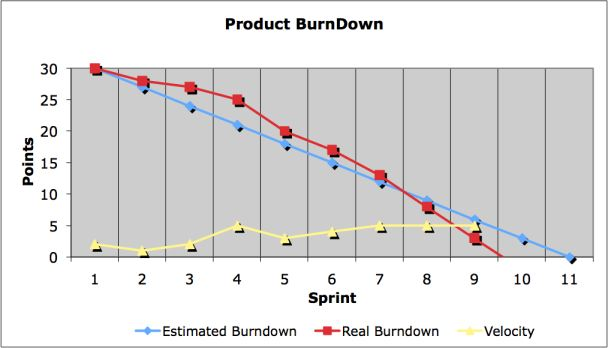
\includegraphics[width=0.5\textwidth]{images/burndown.jpg}
    \caption{Example sprint burndown chart}
\end{figure}

\subsection{Sprint Retrospective}
Upon completion of a sprint, a scrum meeting shall take place for which all team members must be present. This meeting's purpose shall be to determine what goals are being most effectively accomplished and which ones need resources reallocated, or labor redistributed.

\subsection{Individual Status Reports}
During each sprint, each team member will be responsible for logging their individual amounts of work performed for each task in the individual status report. These cannot be changed by any team member other than the one whose name appears at the top. These reports will be presented at the Spring Retrospective. They cannot be changed after this presentation.

\subsection{Engineering Notebooks}
Engineering notebooks will be kept by every member of the team. Inside the notebooks will be documentation of all work, progress, and details for the project done by that individual. Each member is to keep their own notebook with their own progress made on the project. Updates to the notebooks will be done by the owner of the notebook whenever progress is made or at their convenience.   

\subsection{Closeout Materials}
Materials detailing the usage and support of product.

\subsubsection{System Prototype}
System prototype will be developed by the team when the proper components arrive. Prototype will be used for testing and debugging purposes before the final product is created. This prototype will be stored at the Senior Design Lab and handled by the team responsible for the project. Updates will be made based on functional needs. 

\subsubsection{Project Poster}
Project poster will be developed at the time of presentation. Team members will each contribute on poster at the time of need. Poster will give short description small preview of what the product can do. 

\subsubsection{Web Page}
Web page over project will be brief and short. It will showcase the product, functionalities, and descriptions on the project. Updates will be made to correspond with updates to the project.

\subsubsection{Demo Video}
A demo video will be made to showcase product. The video will show basic functionalities and basic usage of the system. Video will be stored on web page. No plans for updating video unless product gets new update. 

\subsubsection{Source Code}
Source code over the project will be done by all members of the team. Storage of the code will be done through Github repositories. Source code will be written to accommodate for the functionalities of the project. The code will be written and maintained by all team members and updated accordingly to fit the needed functionalities over the course of the project. 

\subsubsection{Source Code Documentation}
Source code documentation will be done by the individual responsible for writing that section of the code. Documentation will explain functionalities of the code written and the various details of the code in the event that someone needs to modify it. Documentations will be stored with the source code itself. Updates will be done whenever the source code itself is updated. 

\subsubsection{Hardware Schematics}
\begin{figure}[h!]
    \centering
    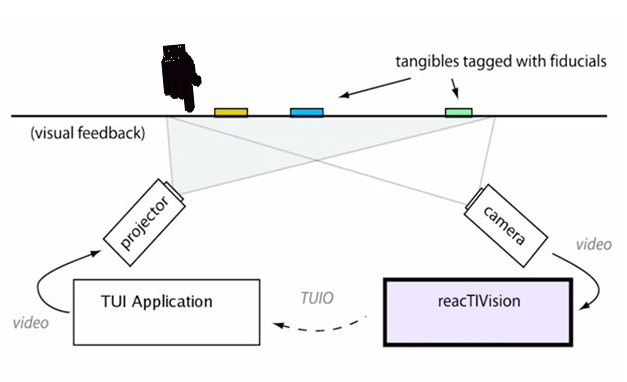
\includegraphics[width=0.5\textwidth]{images/Diagram.jpg}
\end{figure}
A camera provides a real time video stream to reacTIVision. Then the source images have been encoded into the fiducial symbol with an unique ID number. TUIO is a communication protocol of reacTIVision that was designed to encode and transmit the attributes of tangible objects on a table's surface. In order to provide fast and reliable communication with local and remote client applications, TUIO defines a set of OSC (Open Sound Control) messages. These messages encode the fiducials' position, presence and transmit this data to the client applications. On the client side, these messages are decoded to add, update or remove events corresponding to the physical actions that have been applied to each fiducial marker.

\subsubsection{CAD files}
Coner brackets for table
\begin{figure}[h!]
    \centering
    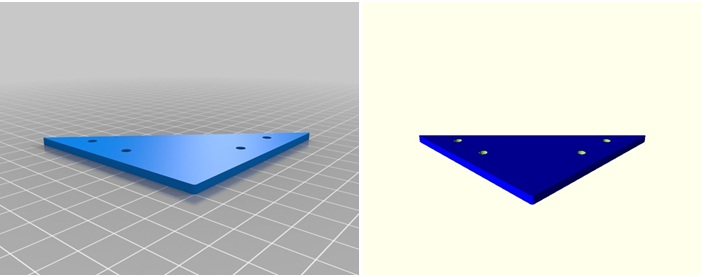
\includegraphics[width=0.5\textwidth]{images/corner_bracket.jpg}
\end{figure}

\subsubsection{Installation Scripts}
\subsubsection{Hardware Installation}
A camera and a projector with wide angle lenses need to be placed underneath the table, so they can both cover the entire surface. The table's surface should be transparent, such as sanded glass with a blurring coating. To achieve a blurring surface, we need to place a sheet of ordinary tracing paper on the table. Also we should have a matte finish on the lower side of surface to avoid direct reflections of the projector lamp. 

\subsubsection{User Manual}
The user manual will be written and documented by a member of the interactive display table team. The member will show knowledge and understanding of how to use the table as well as intricacies of the table that may need to be documented. The user manual itself will detail how to use the table, purpose of table, any various features and explanations on what each part does. Updates to the user manual will be made accordingly with updates done to the product. 

\newpage

%%% References
\bibliographystyle{plain}
\bibliographystyle{reference/IEEEtran_custom}
\bibliography{reference/refs}{}

\end{document}
